\documentclass[aspectratio=169]{beamer} % O parâmetro aspectratio com valar 16:9 deixa o slide em widescreen

\usepackage[brazil]{babel}
\usepackage[utf8]{inputenc}
\usepackage[T1]{fontenc}
\usepackage{listings}
\usepackage{textcomp}

\usetheme{Madrid}
\setbeamertemplate{navigation symbols}{}

\lstset{
language=html,
upquote=true,
basicstyle=\ttfamily\tiny,
backgroundcolor=\color{white},
keywordstyle=\color{blue}\bfseries,
stringstyle=\color{red},
commentstyle=\color{green},
%morecomment=[s][\color{green}]{/**}{*/},
showspaces=false,
showstringspaces=false,
morekeywords={None,self,__init__,True,False},
literate=
{á}{{\'a}}1
{Á}{{\'A}}1
{à}{{\`a}}1 
{À}{{\`A}}1
{â}{{\^a}}1 
{Â}{{\^A}}1
{ã}{{\~a}}1
{Ã}{{\~A}}1
{ä}{{\"a}}1
{Ä}{{\"A}}1
{é}{{\'e}}1
{É}{{\'E}}1
{è}{{\`e}}1
{È}{{\`E}}1
{ê}{{\^e}}1
{Ê}{{\^E}}1
{ẽ}{{\~e}}1
{Ẽ}{{\~E}}1 
{ë}{{\"e}}1
{Ë}{{\"E}}1
{í}{{\'i}}1
{Í}{{\'I}}1
{ì}{{\`i}}1
{Ì}{{\`I}}1
{î}{{\^i}}1
{Î}{{\^I}}1
{ĩ}{{\~i}}1
{Ĩ}{{\~I}}1
{ï}{{\"i}}1
{Ï}{{\"I}}1
{ó}{{\'o}}1
{Ó}{{\'O}}1
{ò}{{\`o}}1
{Ò}{{\`O}}1
{ô}{{\^o}}1
{Ô}{{\^O}}1
{õ}{{\~o}}1
{Õ}{{\~O}}1
{ö}{{\"o}}1
{Ö}{{\"O}}1
{ú}{{\'u}}1
{Ú}{{\'U}}1
{ù}{{\`u}}1
{Ù}{{\`U}}1
{û}{{\^u}}1
{Û}{{\^U}}1
{ũ}{{\~u}}1
{Ũ}{{\~U}}1
{ü}{{\"u}}1
{Ü}{{\"U}}1
{ç}{{\c{c}}}1
{Ç}{{\c{C}}}1
}

\title[HTML]{HTML}

\author[Diego S. C. Nascimento]{Diego Silveira Costa Nascimento}

\institute[IFRN]{
Instituto Federal de Educação, Ciência e Tecnologia do Rio Grande do Norte\\
diego.nascimento@ifrn.edu.br
}

\date[\today]{\today}

\begin{document}

\begin{frame}[plain]
	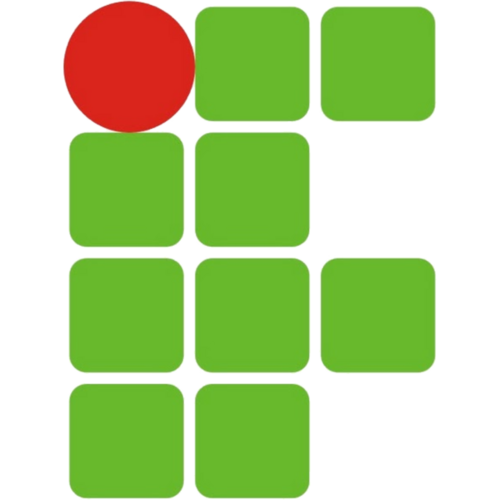
\includegraphics[scale=0.2]{img/IFRN}
	\titlepage
\end{frame}

\logo{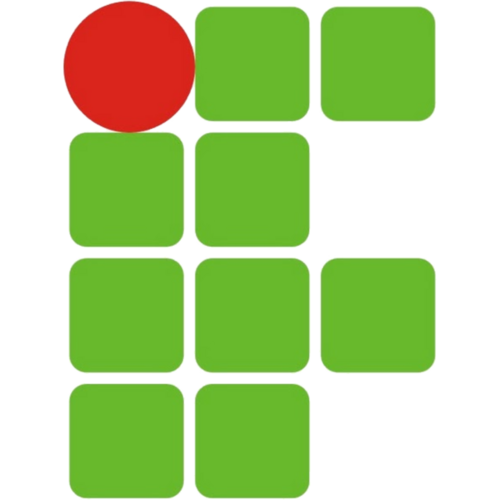
\includegraphics[scale=0.1]{img/IFRN}}

\begin{frame}
	\frametitle{Ementa}
  	\tableofcontents
\end{frame}

\AtBeginSection[]{
	\begin{frame}
		\frametitle{Ementa do Curso}
		\tableofcontents[currentsection]
	\end{frame}
}

\section{Introdução}

\begin{frame}
	\frametitle{HTML}
	
	\begin{itemize}
		\item É que uma linguagem de marcação fundamental para criar páginas web;
		\item É um acrônimo para \underline{H}yperText \underline{M}arkup \underline{L}anguage;
		\item Não é uma linguagem de programação; e
		\item Foi criado 1991 pelo cientista Tim Berners-Lee.
	\end{itemize}
\end{frame}

\begin{frame}[fragile]
\frametitle{Como funciona?}

\begin{itemize}
	\item Utiliza tags para envolver e definir o tipo de conteúdo;
	\item As tags são palavras-chave, geralmente dentro de sinais de menor e maior: \structure{< >}; e
	\item Pode ser escrito em qualquer editor de texto, e salvo no formato \structure{.html}.
\end{itemize}\vfill

\begin{exampleblock}{Exemplos}
	\begin{lstlisting}
<!DOCTYPE html>

<html></html>

<meta>

<body></body>

<img>
	\end{lstlisting}
\end{exampleblock}
\end{frame}

\begin{frame}[fragile]
	\frametitle{Primeira página}
		
	\begin{exampleblock}{Exemplo}
		\begin{lstlisting}
<!DOCTYPE html>
<html>

	<head>
		<meta charset="UTF-8">
		<title>Minha página</title>
	</head>

	<body>
		Olá, mundo!
	</body>

</html>
		\end{lstlisting}
	\end{exampleblock}
\end{frame}

\begin{frame}[fragile]
	\frametitle{Cabeçalho}
	
	\begin{itemize}
		\item As tags de cabeçalho \structure{<h1>} a \structure{<h6>} são elementos essenciais para estruturar e organizar o conteúdo de uma página; e
		\item O tamanho do cabeçalho aparece em ordem decrescente para cada par de tags.
	\end{itemize}\vfill
	
	\begin{exampleblock}{Exemplo}
		\begin{lstlisting}
<h1>Título 1</h1>
<h2>Título 2</h2>
<h3>Título 3</h3>
<h4>Título 4</h4>
<h5>Título 5</h5>
<h6>Título 6</h6>
		\end{lstlisting}
	\end{exampleblock}
\end{frame}

\begin{frame}[fragile]
	\frametitle{Parágrafo}
	
	\begin{itemize}
		\item A tag \structure{<p>} é usada para definir um parágrafo de texto; e
		\item É um elemento de bloco, o que significa que ocupa toda a largura disponível.
	\end{itemize}\vfill
	
	\begin{exampleblock}{Exemplo}
		\begin{lstlisting}
<p>O IFRN é uma instituição pública de ensino, fundada em 1909, que oferece educação profissional e tecnológica
gratuita em diferentes níveis (básico, técnico, superior e pós-graduação), com 22 campi em todo o estado. Seu 
objetivo é formar cidadãos e profissionais por meio da articulação entre ciência, cultura, trabalho e tecnologia,
promovendo a inclusão social e o desenvolvimento do Rio Grande do Norte.</p>
		\end{lstlisting}
	\end{exampleblock}
\end{frame}

\begin{frame}[fragile]
	\frametitle{Quebra de linha}
	
	\begin{itemize}
		\item A tag  \structure{<br>} serve para inserir uma quebra de linha simples no texto; e
		\item \alert{Não inicia um novo parágrafo}.
	\end{itemize}\vfill
	
	\begin{exampleblock}{Exemplo}
		\begin{lstlisting}
<p>O IFRN é uma instituição pública de ensino, fundada em 1909, <br>
que oferece educação profissional e tecnológicagratuita em diferentes <br>
níveis (básico, técnico, superior e pós-graduação), com 22 campi em todo <br> 
o estado. Seu objetivo é formar cidadãos e profissionais por meio da <br> 
articulação entre ciência, cultura, trabalho e tecnologia, promovendo a <br>
inclusão social e o desenvolvimento do Rio Grande do Norte.</p>
		\end{lstlisting}
	\end{exampleblock}
\end{frame}

\begin{frame}[fragile]
	\frametitle{Linha horizontal}
	
	\begin{itemize}
		\item A tag \structure{<hr>} é usada para criar uma linha horizontal; e
		\item Funciona como um divisor temático entre o conteúdo de uma página.
	\end{itemize}\vfill
	
	\begin{exampleblock}{Exemplo}
		\begin{lstlisting}
<h1>IFRN</h1>

<hr>

<p>O IFRN é uma instituição pública de ensino, fundada em 1909, que oferece educação profissional e tecnológica
gratuita em diferentes níveis (básico, técnico, superior e pós-graduação), com 22 campi em todo o estado. Seu 
objetivo é formar cidadãos e profissionais por meio da articulação entre ciência, cultura, trabalho e tecnologia,
promovendo a inclusão social e o desenvolvimento do Rio Grande do Norte.</p>
		\end{lstlisting}
	\end{exampleblock}
\end{frame}

\begin{frame}[fragile]
	\frametitle{Imagem}
	
	\begin{itemize}
		\item A tag \structure{<img>} é usada para incorporar imagens em uma página da web;
		\item Precisa dos atributos \structure{src}, \structure{width} e \structure{height}.
	\end{itemize}\vfill
	
	\begin{exampleblock}{Exemplo}
		\begin{lstlisting}
<img src="IFRN.png" width="200" height="200" />
		\end{lstlisting}
	\end{exampleblock}
\end{frame}

\section{Listas}

\begin{frame}
	\frametitle{Listas}
	
	\begin{itemize}
		\item São essenciais para estruturar conteúdo de forma legível e organizada na web;
		\item Há três tipos diferentes de listas: 
		\begin{itemize}
			\item Lista não ordenadas;
			\item Lista ordenadas; e
			\item Lista de definição.
		\end{itemize}
	\end{itemize}
\end{frame}

\begin{frame}[fragile]
	\frametitle{Lista não ordenada}
	
	\begin{itemize}
		\item A tag principal é \structure{<ul>}, e o  item da lista é \structure{<li>};
		\item Ideal para itens onde a ordem não importa.
	\end{itemize}\vfill
	
	\begin{exampleblock}{Exemplo}
		\begin{lstlisting}
<ul>
	<li>Item A</li>
	<li>Item B</li>
	<li>Item C</li>
</ul>
		\end{lstlisting}
	\end{exampleblock}
\end{frame}

\begin{frame}[fragile]
	\frametitle{Lista ordenada}
	
	\begin{itemize}
		\item A tag principal é \structure{<ol>}, e o item da lista é \structure{<li>}; e.
		\item Ideal para conteúdo onde a sequência ou ordem é importante (passos, rankings, instruções)
	\end{itemize}\vfill
	
	\begin{exampleblock}{Exemplo}
		\begin{lstlisting}
<ol>
	<li>Primeiro Passo</li>
	<li>Segundo Passo</li>
	<li>Terceiro Passo</li>
</ol>
		\end{lstlisting}
	\end{exampleblock}
\end{frame}

\begin{frame}[fragile]
	\frametitle{Lista de definição}
	
	\begin{itemize}
		\item  A tag principal é \structure{<dl>}, e o termo a definir é \structure{<dt>}, para a definição/descrição usa-se \structure{<dd>}; e
		\item Utilizada para criar um glossário ou listar pares de Termo/Descrição ou Nome/Valor.
	\end{itemize}\vfill
	
	\begin{exampleblock}{Exemplo}
		\begin{lstlisting}
<dl>
	<dt>HTML</dt>
		<dd>Linguagem de Marcação de Hipertexto.</dd>
	<dt>CSS</dt>
		<dd>Folhas de Estilo em Cascata, usadas para estilizar elementos.</dd>
</dl>
		\end{lstlisting}
	\end{exampleblock}
\end{frame}

\section{Tabela}

\begin{frame}[fragile]
	\frametitle{Tabela}
	
	\begin{itemize}
		\item  A tag \structure{<table>} define uma tabela para estruturar dados;
		\item É organizada por linhas (\structure{<tr>}); e 
		\item E cada linha possui células (\structure{<td>} para dados, \structure{<th>} para cabeçalho)
	\end{itemize}
	
	\begin{exampleblock}{Exemplo}
	\begin{lstlisting}
<table>
	<caption>Título da Tabela</caption>
	<thead>
		<tr>
			<th>Cabeçalho 1</th>
			<th>Cabeçalho 2</th>
		</tr>
	</thead>
	<tbody>
		<tr>
			<td>Dado 1</td>
			<td>Dado 2</td>
		</tr>
	</tbody>
</table>
	\end{lstlisting}
\end{exampleblock}
\end{frame}

\section{Hiperlink}

\begin{frame}[fragile]
	\frametitle{Link}
	
	\begin{itemize}
		\item A tag \structure{<a></a>} cria links que permitem navegar entre páginas;
		\item O atributo \structure{href} define o caminho;
		\item Um caminho pode ser:
		\begin{itemize}
			\item Absoluto -- https://portal.ifrn.edu.br/; ou
			\item Relativo -- sobre.html;
		\end{itemize}
		\item O atributo \structure{target}="\_blank" abre a página em uma nova aba.
	\end{itemize}\vfill
	
	\begin{exampleblock}{Exemplo}
		\begin{lstlisting}
	<a href="https://portal.ifrn.edu.br/">Google</a>
		\end{lstlisting}
	\end{exampleblock}
\end{frame}

\section{Formulário}

\begin{frame}[fragile]
	\frametitle{Formulário}
	
	\begin{itemize}
		\item A tag \structure{<form></form>} define um formulário;
		\item Os elementos de entrada de dados, podem ser: caixas de texto, botões de rádio, caixas de seleção ou botões;
		\item O atributo \structure{action} corresponde ao endereço (URL) para onde os dados serão enviados após o envio; e
		\item O \structure{method} corresponde ao método HTTP (\structure{GET} ou \structure{POST}) usado para enviar os dados. 
	\end{itemize}\vfill
	
	\begin{exampleblock}{Exemplo}
		\begin{lstlisting}
<form action="salvar.php" method="POST">

</form>
		\end{lstlisting}
	\end{exampleblock}
\end{frame}

\end{document}